\chapter{Heading of Test Chapter 2}\label{testchaptertwo}

This is another chapter of the book.

\begin{Shaded}
\begin{Highlighting}[]
\KeywordTok{plot}\NormalTok{(faithful, }\DataTypeTok{col =} \StringTok{"blue"}\NormalTok{, }\DataTypeTok{main =} \StringTok{"Eruptions of Old Faithful"}\NormalTok{)}
\end{Highlighting}
\end{Shaded}

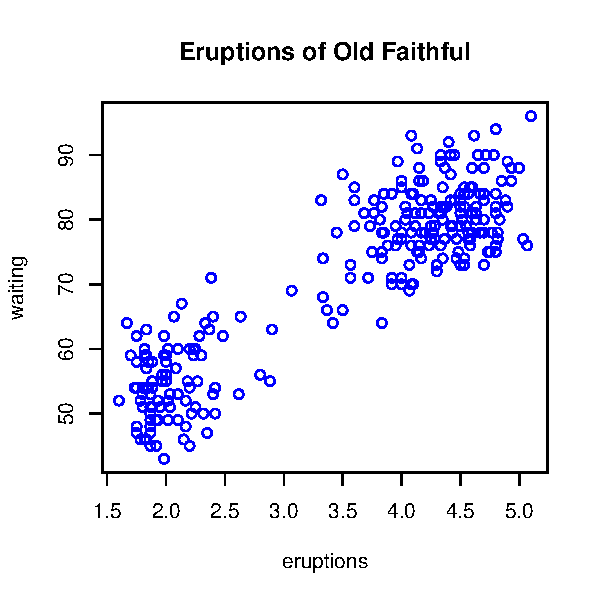
\includegraphics{figures/old_faithful-1.pdf}

Figure 2.1: Eruptions of Old Faithful

This is a \emph{very} basic plot (Figure 2.1). But it's easy to make
very elegant and useful visuaisations with R, thanks to the numerous
accessible books on the topic (Chang, 2012; Murrell, 2011; Wickham,
2009)

\section*{References}
\addcontentsline{toc}{section}{References}

Chang, W. (2012). \emph{R graphics cookbook}. `` O'Reilly Media, Inc.''

Murrell, P. (2011). \emph{R graphics}. CRC Press.

Wickham, H. (2009). \emph{Ggplot2: Elegant graphics for data analysis}.
Springer Science \& Business Media.
